\documentclass[11pt, a4paper]{article}
\usepackage{geometry}
\usepackage[parfill]{parskip}
\usepackage{graphicx}
\usepackage{amsmath}
\usepackage{enumerate}

\usepackage{charter}

\title{Huiswerk 4 \\ IB0402 Logica, verzamelingen en relaties}
\author{Harman Singh}
\date{Month Day, Year}

\begin{document}
\maketitle

\pagebreak
\section*{Opgave 11}

\subsection*{A}

Deze zijn samenhangen (elk punt in de graaf is bereikbaar vanaf elk ander punt) en vlak (geen kruisende lijnen):

\begin{itemize}
	\item de twee-en-een-na-laatste op de bovenste rij
	\item de eerste twee op de onderste rij
\end{itemize}

De opgave zegt dat er 6 zijn, maar ik denk dat er enkel 4 zijn. Alle vier op de onderste rij zijn samenhangend, maar de laatste twee bevat kruisende lijnen wat betekent dat ze niet vlak zijn.


\subsection*{B}

Ik ga hier links naar rechts, van boven naar beneden.

\textbf{graaf 1}
\begin{itemize}
	\item $v$, aantal punten \hfill 4
	\item $e$, aantal lijnen \hfill 3
	\item $f$, aantal gebieden \hfill 1 (gewoon het vlak)
	\item $v-e+f$ \hfill $\boxed{4 - 3 + 1 = 2}$
\end{itemize}



\textbf{graaf 2}
\begin{itemize}
	\item $v$ = 4; $e$ = 3; $f$ = 1 (gewoon het vlak)
	\item $v-e+f$ \hfill $\boxed{4 - 3 + 1 = 2}$
\end{itemize}


\textbf{graaf 3}
\begin{itemize}
	\item $v$ = 4; $e$ = 4; $f$ = 2 (de vierkant binnen, en het gebied dat om de graaf heen ligt)
	\item $v-e+f$ \hfill $\boxed{4 - 4 + 2 = 2}$
\end{itemize}


\textbf{graaf 4}
\begin{itemize}
	\item $v$ = 4; $e$ = 5; $f$ = 3 (de driehoek binnen, en het gebied dat om de graaf heen ligt)
	\item $v-e+f$ \hfill $\boxed{4 - 5 + 3 = 2}$
\end{itemize}



\pagebreak
\subsection*{C}

Als $f$ gelijk is aan 1, dan betekent het dat er geen gesloten gebieden zijn. Dit betekent dat je nooit een cykel kan vormen en dus altijd 1 minder lijn nodig zal hebben dan er punten zijn.

Bijvoorbeeld om 4 punten te verbinden zonder er een vierkant van te maken (want dit zou betekent dat $f>1$), heb je enkel 3 lijnen nodig.

Dit soort graaf wordt een \textit{boom} genoemd


\section*{Opgave 12}



\subsection*{A}

Ik los eerst op naar $y$, dus $x^2 + 2y = 3$ wordt:

\[
	2y = 3 - x^2 
\]

\[
	\equiv y = \frac{3 - x^2}{2}
\]


Deze functie ziet er zo uit:

\begin{center}
	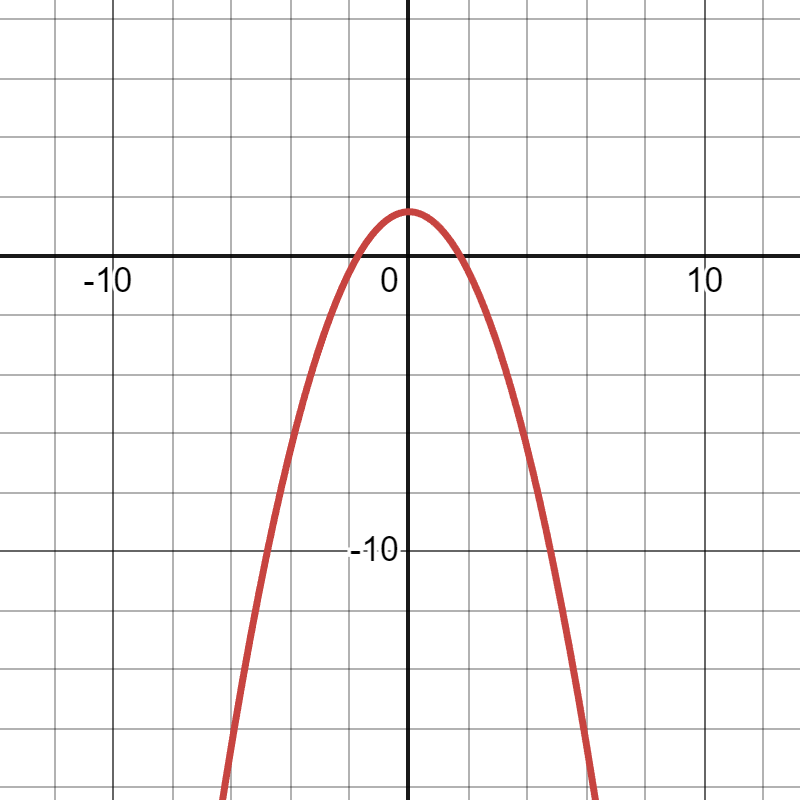
\includegraphics[width=0.5\textwidth]{opgave12_a.png}
\end{center}

Voor elke waarde van $x$ kan je een waarde van $y$ uitrekenen, dus dit is een functie van $x$ naar $y$.

Bijvoorbeeld, als $x = 3$, dan is $y = \frac{3 - (3^2)}{2} = \frac{3 - 9}{2} = \frac{-6}{2} = -3$.


\subsection*{B}

Hier los ik op naar $x$, dus $y^2 + 2x = 3$ wordt:

\[
	2x = 3 - y^2
\]

\[
\equiv x = \frac{3 - y^2}{2}
\]


Deze functie ziet er zo uit:

\begin{center}
	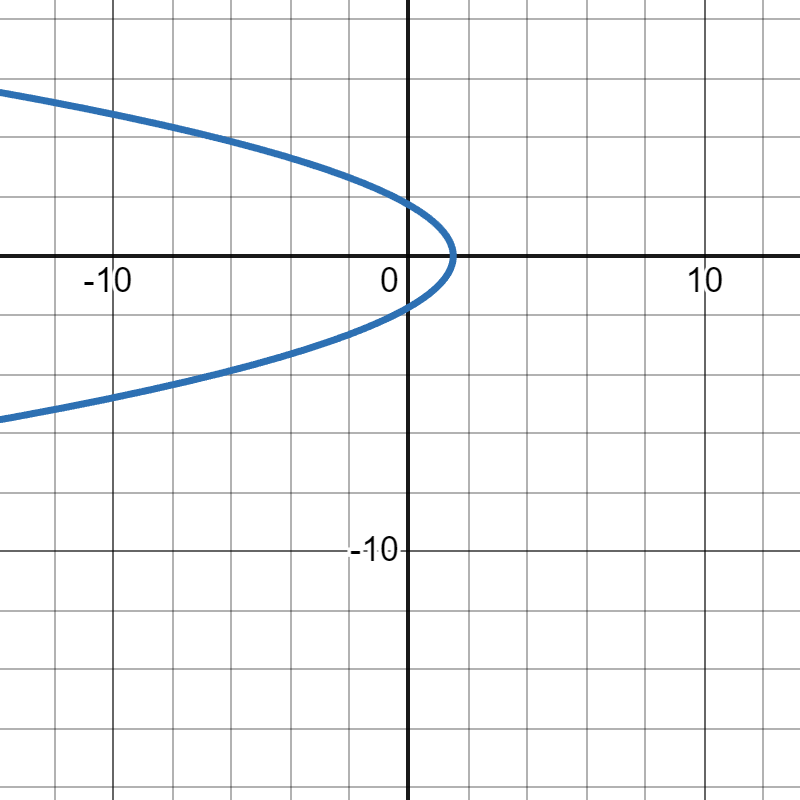
\includegraphics[width=0.5\textwidth]{opgave12_b.png}
\end{center}

Voor elke waarde van $y$ kan je een waarde van $x$ uitrekenen, dus dit is een functie van $y$ naar $x$.

Bijvoorbeeld, als $y = 3$, dan is $x = \frac{3 - (3^2)}{2} = \frac{3 - 9}{2} = \frac{-6}{2} = -3$.

\textbf{Maar}, als je $x$ als invoer neemt, dan is dit geen functie, omdat je voor sommige waarden van $x$ twee mogelijke waarden van $y$ krijgt, bijvoorbeeld als $x = 1$, dan is $y^2 + 2(1) = 3$ of $y^2 = 1$ wat betekent dat $y = 1$ of $y = -1$.

\section*{Opgave 13}

\subsection*{A}

\[
f((4,7)) = (4+7, 7) = (11, 7)
\]

\[
g((11,4)) = (11-4, 4) = (7, 4)
\]


\subsection*{B}

$g \circ f$ betekent we eerst $f$ toepassen, en daarna $g$ op het resultaat van $f$.

Dus
\[
f((x,y)) = (x+y, x)
\]

\[
g(f(x,y)) = g((x+y,x)) = ((x+y)-x,x) = (y,x)
\]

Dus eigenlijk draaien we de twee elementen om.

\subsubsection*{(2,2)}

\[
g(f((2,2))) = \boxed{(2, 2)}
\]

\subsubsection*{(3,5)}
\[
g(f((3,5))) = \boxed{(5, 3)}
\]


\subsubsection*{(4,1)}
\[
	g(f((4,1))) = \boxed{(1, 4)}
\]


\subsection*{C}

Een functie $h$ die hetzelfde doet als $g \circ f$ is:

\[
	\boxed{h((x,y)) = (y,x)}
\]


\subsection*{D}
\ldots



\ldots
\end{document}